\documentclass[10pt,ignorenonframetext,]{beamer}
\setbeamertemplate{caption}[numbered]
\setbeamertemplate{caption label separator}{: }
\setbeamercolor{caption name}{fg=normal text.fg}
\beamertemplatenavigationsymbolsempty
\usepackage{lmodern}
\usepackage{amssymb,amsmath}
\usepackage{ifxetex,ifluatex}
\usepackage{fixltx2e} % provides \textsubscript
\ifnum 0\ifxetex 1\fi\ifluatex 1\fi=0 % if pdftex
  \usepackage[T1]{fontenc}
  \usepackage[utf8]{inputenc}
\else % if luatex or xelatex
  \ifxetex
    \usepackage{mathspec}
  \else
    \usepackage{fontspec}
  \fi
  \defaultfontfeatures{Ligatures=TeX,Scale=MatchLowercase}
\fi
\usetheme[]{metropolis}
% use upquote if available, for straight quotes in verbatim environments
\IfFileExists{upquote.sty}{\usepackage{upquote}}{}
% use microtype if available
\IfFileExists{microtype.sty}{%
\usepackage{microtype}
\UseMicrotypeSet[protrusion]{basicmath} % disable protrusion for tt fonts
}{}
\newif\ifbibliography
\hypersetup{
            pdftitle={Combining multiple sources of information with Markov melding},
            pdfauthor={Andrew Manderson},
            pdfborder={0 0 0},
            breaklinks=true}
\urlstyle{same}  % don't use monospace font for urls

% Prevent slide breaks in the middle of a paragraph:
\widowpenalties 1 10000
\raggedbottom

\AtBeginPart{
  \let\insertpartnumber\relax
  \let\partname\relax
  \frame{\partpage}
}
\AtBeginSection{
  \ifbibliography
  \else
    \let\insertsectionnumber\relax
    \let\sectionname\relax
    \frame{\sectionpage}
  \fi
}
\AtBeginSubsection{
  \let\insertsubsectionnumber\relax
  \let\subsectionname\relax
  \frame{\subsectionpage}
}

\setlength{\parindent}{0pt}
\setlength{\parskip}{6pt plus 2pt minus 1pt}
\setlength{\emergencystretch}{3em}  % prevent overfull lines
\providecommand{\tightlist}{%
  \setlength{\itemsep}{0pt}\setlength{\parskip}{0pt}}
\setcounter{secnumdepth}{0}
\usepackage{amsmath}
% I always seem to need tikz for something
\usepackage{tikz}
\usetikzlibrary{positioning, shapes, intersections, through, backgrounds, fit, decorations.pathmorphing, angles, quotes}

% \usepackage{setspace}
% \onehalfspacing

\usepackage{lineno}
% \linenumbers

% required for landscape pages. beware, they back the build very slow.
\usepackage{pdflscape}

% table
\usepackage{longtable}
\usepackage{booktabs}
\usepackage{caption}

% \usepackage[colorlinks=true, urlcolor=citecolor, linkcolor=citecolor, citecolor=citecolor]{hyperref}

% cross out math
\usepackage[makeroom]{cancel}

\usepackage{color}
\definecolor{myredhighlight}{RGB}{180, 15, 32}
\definecolor{mydarkblue}{RGB}{0, 33, 79}
\definecolor{mymidblue}{RGB}{44, 127, 184}
\newcommand{\semitransp}[2][35]{\color{fg!#1}#2}

% beamer things
\setbeamercolor{frametitle}{bg=black}
\setbeamerfont{footnote}{size=\tiny}
\widowpenalties 1 150
\setbeamertemplate{page number in head/foot}{}

\setcounter{secnumdepth}{3}

% pd stands for: probability distribution and is useful to distringuish
% marignals for probabilities specifically p(p_{1}) and the like.
\newcommand{\pd}{\text{p}}
\newcommand{\q}{\text{q}}
\newcommand{\w}{\text{w}}
\newcommand{\pdr}{\text{r}}
\newcommand{\pdrh}{\hat{\text{r}}}

% melding
\newcommand{\ppoolphi}{\pd_{\text{pool}}(\phi)}

% the q(x)w(x), "weighted target" density 
% for the moment I'm going to call it s(x), as that is the next letter of the 
% alphabet. Can change it later
\newcommand{\s}{\text{s}}
% direct density estimate - replaces lambda.
\newcommand{\ddest}{\text{s}}

% constants - usually sizes of things
\newcommand{\Nx}{N}
\newcommand{\Nnu}{\text{N}_{\text{nu}}}
\newcommand{\Nde}{\text{N}_{\text{de}}}
\newcommand{\Nmc}{\text{N}_{\text{mc}}}
\newcommand{\Nw}{W}
\newcommand{\Nm}{M}

% locales - could switch to x and x'
\newcommand{\xnu}{x_{\text{nu}}}
\newcommand{\xde}{x_{\text{de}}}
\newcommand{\phinu}{\phi_{\text{nu}}}
\newcommand{\phide}{\phi_{\text{de}}}

% sugiyama stuff
\newcommand{\pdnu}{\pd_{\text{nu}}}
\newcommand{\pdde}{\pd_{\text{de}}}


% indices 
\newcommand{\wfindex}{w}
\newcommand{\sampleindex}{n}
\newcommand{\modelindex}{m}

\title{Combining multiple sources of information with Markov melding}
\subtitle{Examples, challenges, and (partial) solutions}
\author{Andrew Manderson}
\institute{MRC Biostatistics Unit, University of Cambridge \& The Alan Turing
Institute.}
\date{2020-01-28}

\begin{document}
\frame{\titlepage}

\begin{frame}{Model criticism - 1}

\begin{center}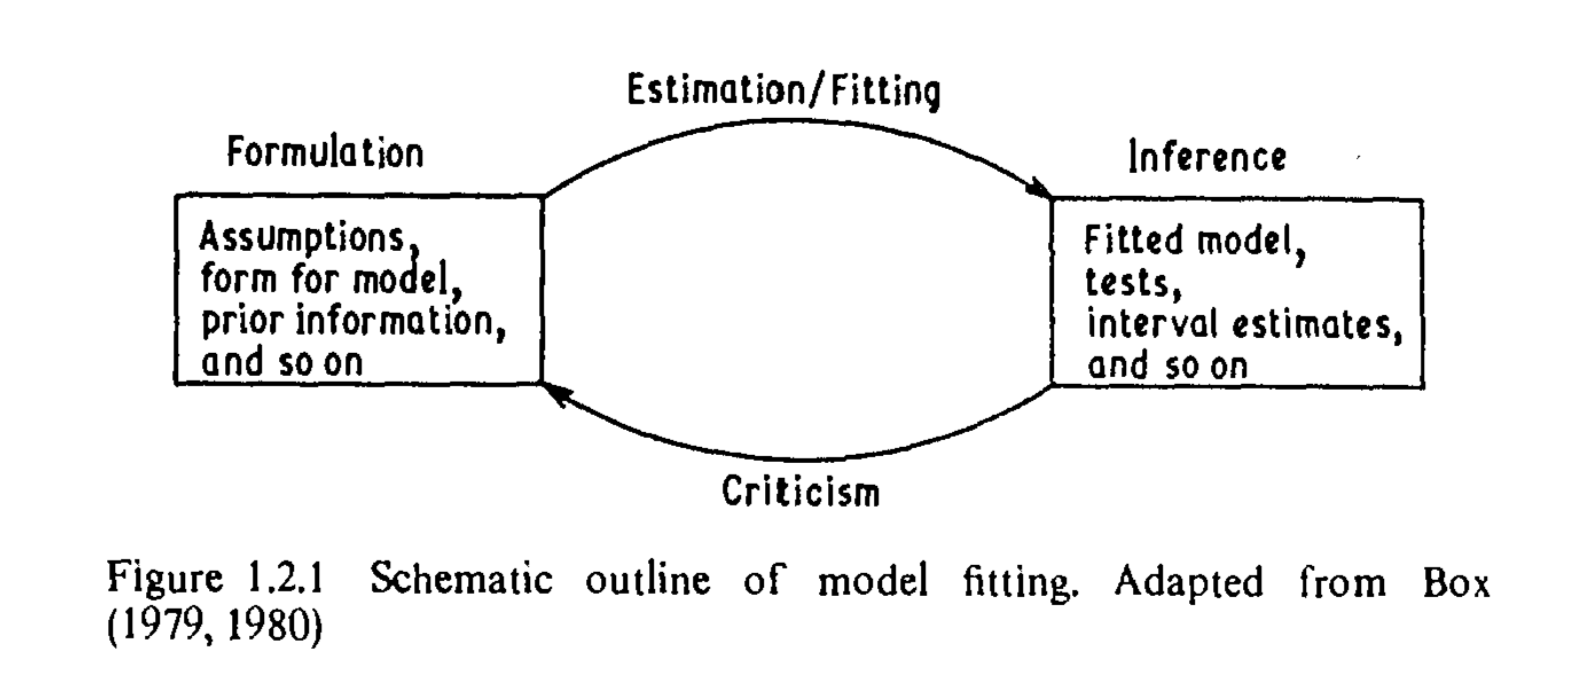
\includegraphics[width=1\linewidth]{figures/modelling-process} \end{center}

\begin{itemize}
\tightlist
\item
  From Cook and Weisberg (1982), but really from Box (1979; 1980)
\end{itemize}

\end{frame}

\begin{frame}{Model criticism - 2}

\begin{center}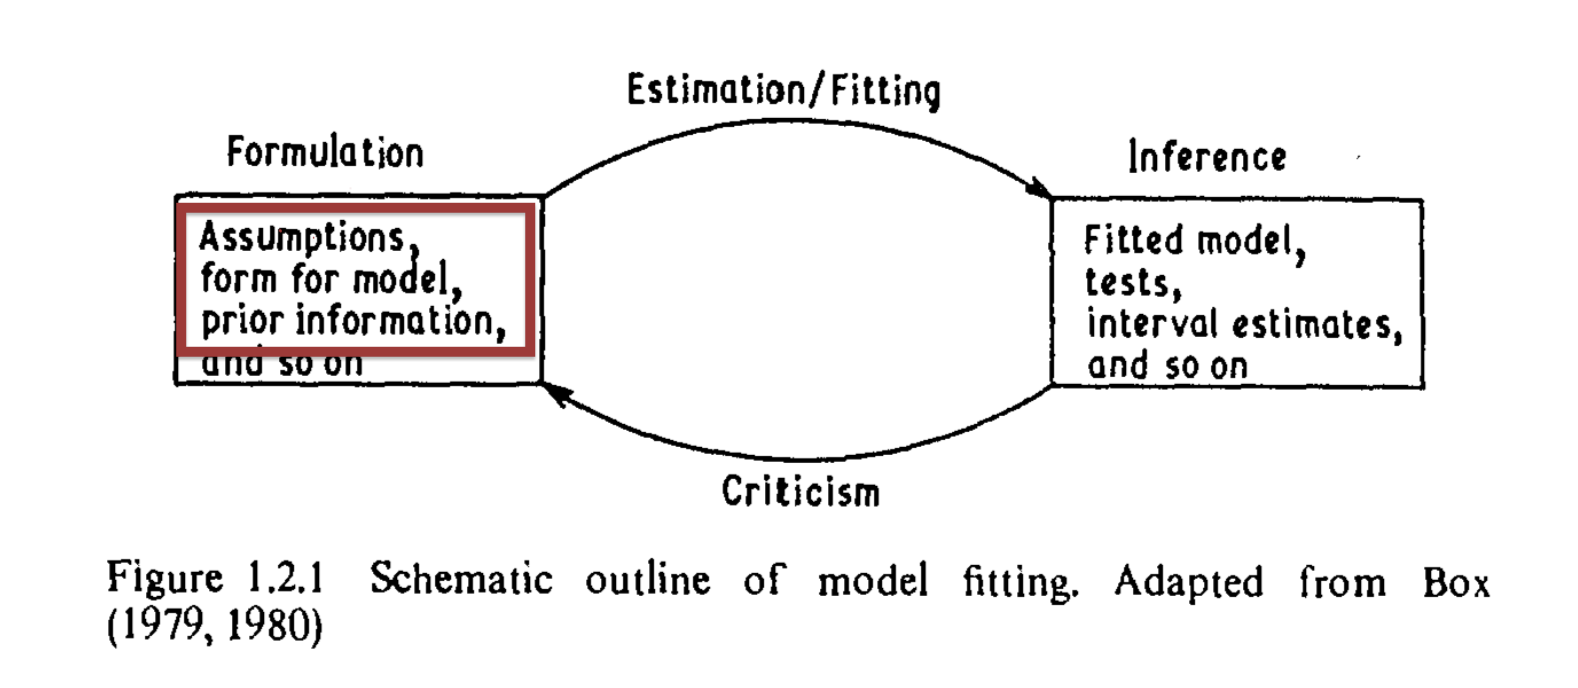
\includegraphics[width=1\linewidth]{figures/modelling-process-2} \end{center}

\begin{itemize}
\tightlist
\item
  From Cook and Weisberg (1982), but really from Box (1979; 1980)
\item
  Non-linear increase in difficulty when
  \(\textcolor{myredhighlight}{n, p \to \infty}\)
\end{itemize}

\end{frame}

\begin{frame}{A complex applied analysis}

\begin{center}
\includegraphics[width=1\linewidth]{figures/2014_Presanis_melding-h1n1-example} \end{center}

\begin{itemize}
\tightlist
\item
  5 sources of data, each idiosyncratic.

  \begin{itemize}
  \tightlist
  \item
    Some known to be biased in particular directions
  \item
    Different levels of aggregation, national / hospital specific data
  \end{itemize}
\item
  Specifying and critiquing a joint model for all of this?
\item
  Will return to a simplified version
\end{itemize}

\end{frame}

\begin{frame}{Statistical modelling}

\begin{center}
\begin{tikzpicture}[node distance = 2cm, thick, state/.style={circle, draw, minimum width = 1.5cm, align = center}]
  % nodes
  \node [state] (data) {Data: \\ $Y$};
  \node [state][right = 2.0cm of data] (model) {Model: \\ $\pd(\phi, \psi, Y)$};

  % edges
  \draw [dashed] [->] (model) to [bend right = 70] (data);
  \draw [dashed] [->] (data) to [bend right = 70] (model); 
\end{tikzpicture}
\end{center}

\end{frame}

\begin{frame}{Statistical submodelling}

\begin{center}
\begin{tikzpicture}[node distance = 2cm, thick, state/.style={circle, draw, minimum width = 1.5cm, align = center}]
  % nodes
  \node [state] (data) {$Y_{1}$};
  \node [state, opacity = 0.75][above right = 1.75cm of data.center] (data1) {$Y_{2}$};
  \node [state, opacity = 0.5][above right = 1.25cm of data1.center] (data2) {$Y_{3}$};
  \node [state, opacity = 0.25][above right = 1.25cm of data2.center] (data3) {$Y_{4}$};
  
  \node [state][right = 2.0cm of data] (model) {  $\pd_{1}(\phi, \psi_{1}, Y_{1})$};
  \node [state, opacity = 0.3][above right = 1.75cm of model.center] (model1) {$\pd_{2}(\phi, \psi_{2}, Y_{2})$};
  \node [state, opacity = 0.2][above right = 1.25cm of model1.center] (model2) {$\pd_{3}(\phi, \psi_{3}, Y_{3})$};
  \node [state, opacity = 0.1][above right = 1.25cm of model2.center] (model3) {$\pd_{4}(\phi, \psi_{4}, Y_{4})$};

  % edges
  \draw [dashed] [->] (model) to [bend right = 20] (data);  
  \draw [dashed] [->] (data) to [bend right = 20] (model);  

  \draw [dashed, opacity = 0.3] [->] (model1) to [bend right = 2  0] (data1);
  \draw [dashed, opacity = 0.15] [->] (data1) to [bend right =  20] (model1); 

  \draw [dashed, opacity = 0.2] [->] (model2) to [bend right = 20] (data2);
  \draw [dashed, opacity = 0.2] [->] (data2) to [bend right = 20] (model2); 

  \draw [dashed, opacity = 0.1] [->] (model3) to [bend right = 20] (data3);
  \draw [dashed, opacity = 0.1] [->] (data3) to [bend right = 20] (model3); 
\end{tikzpicture}
\end{center}

\end{frame}

\begin{frame}{Melding based statistical modelling?}

\begin{center}
\begin{tikzpicture}[node distance = 2cm, thick, state/.style={circle, draw, minimum width = 1.5cm}]
  % nodes
  \node [state] (data) {$Y_{1}$};
  \node [state, opacity = 0.9][above right = 1.25cm of data.center] (data1) {$Y_{2}$};
  \node [state, opacity = 0.9][above right = 1.25cm of data1.center] (data2) {$Y_{3}$};
  \node [state, opacity = 0.9][above right = 1.25cm of data2.center] (data3) {$Y_{4}$};
  
  \node [state][right = 2.0cm of data] (model) {$\pd_{1}(\phi, \psi_{1}, Y_{1})$};
  \node [state, opacity = 0.9][above right = 1.25cm of model.center] (model1) {$\pd_{2}(\phi, \psi_{2}, Y_{2})$};
  \node [state, opacity = 0.9][above right = 1.25cm of model1.center] (model2) {$\pd_{3}(\phi, \psi_{3}, Y_{3})$};
  \node [state, opacity = 0.9][above right = 1.25cm of model2.center] (model3) {$\pd_{4}(\phi, \psi_{4}, Y_{4})$};

  \node [rectangle, draw, inner sep = 3pt] [below right = 0.3cm and 1.40cm of model.center] (meld) {$\pd_{\text{meld}} (\phi, \psi_{1}, \psi_{2}, \psi_{3}, \psi_{4}, Y_{1}, Y_{2}, Y_{3}, Y_{4})$};

  % edges
  \draw [dashed] [->] (model) to [bend right = 20] (data);
  \draw [dashed, opacity = 0.05] [->] (data) to [bend right = 20] (model); 

  \draw [dashed, opacity = 1] [->] (model1) to [bend right = 20] (data1);
  \draw [dashed, opacity = 0.05] [->] (data1) to [bend right = 20] (model1); 

  \draw [dashed, opacity = 1] [->] (model2) to [bend right = 10] (data2);
  \draw [dashed, opacity = 0.05] [->] (data2) to [bend right = 10] (model2); 

  \draw [dashed, opacity = 1] [->] (model3) to [bend right = 20] (data3);
  \draw [dashed, opacity = 0.05] [->] (data3) to [bend right = 20] (model3); 

  \draw [->] (meld) to [bend left = 10] (model);
  \draw [->] (meld) to [bend left = 10] (model1);
  \draw [->] (meld) to [bend right = 10] (model2);
  \draw [->] (meld) to [bend right = 10] (model3);
\end{tikzpicture}
\end{center}

\end{frame}

\begin{frame}{\emph{Specification}: Markov melding}

\begin{itemize}
\tightlist
\item
  Markov melding (Goudie et al. 2019) is a method for joining models
  with common component: \(\phi\)
\item
  Ideally we would specify the generative model (For \(M = 2\)
  submodels): \begin{equation*}
  \pd_{\text{meld}} (\phi, \psi_{1}, \psi_{2}, Y_{1}, Y_{2})
  =
  \ppoolphi \,\,
  \pd_{1}(\psi_{1}, Y_{1} \mid \phi) \,\,
  \pd_{2}(\psi_{2}, Y_{2} \mid \phi) 
\end{equation*}
\item
  Submodels developed in isolation, re-express as:
  \begin{equation*}
  \pd_{\text{meld}} (\phi, \psi_{1}, \psi_{2}, Y_{1}, Y_{2})
  =
  \ppoolphi \,\,
  \frac {
    \pd_{1}(\phi, \psi_{1}, Y_{1})
  } {
    \textcolor{myredhighlight}{\pd_{1}(\phi)}
  }
  \,\,
  \frac {
    \pd_{2}(\phi, \psi_{2}, Y_{2})
  } {
    \textcolor{myredhighlight}{\pd_{2}(\phi)}
  }
\end{equation*}
\item
  Analytic form of
  \(\textcolor{myredhighlight}{\pd_{\modelindex}(\phi)}\) often unknown

  \begin{itemize}
  \tightlist
  \item
    Can cause numerical issues in the model fitting process
  \item
    Requires accurate estimation in low probability regions

    \begin{itemize}
    \tightlist
    \item
      We will revisit
    \end{itemize}
  \end{itemize}
\end{itemize}

\end{frame}

\begin{frame}{\emph{Specification}: Notes on the pooled prior}

\(\ppoolphi\) addresses two issues:

\begin{enumerate}
\def\labelenumi{\arabic{enumi}.}
\tightlist
\item
  Necessary because we have two priors for \(\phi\) (Poole and Raftery
  2000) \vspace{0.5cm}
\item
  \(\ppoolphi\) should be appropriate for \(\phi\) under the melded
  model \emph{and} both submodels

  \begin{itemize}
  \tightlist
  \item
    Suggests defining \(\ppoolphi = g(\pd_{1}(\phi), \pd_{2}(\phi))\)
  \item
    Similar problem encountered when experts encode their opinions as
    priors (O'Hagan et al. 2006)

    \begin{itemize}
    \tightlist
    \item
      \(\textcolor{myredhighlight}{\textbf{Log}}\):
      \(\ppoolphi = \pd_{1}(\phi)^{w_{1}} \pd_{2}(\phi)^{w_{2}}\)
    \item
      Linear:
      \(\ppoolphi = {w_{1}}\pd_{1}(\phi) + {w_{2}}\pd_{2}(\phi)\)
      \vspace{0.25cm}
    \item
      Product-of-experts: \(\ppoolphi = \pd_{1}(\phi) \pd_{2}(\phi)\)
      (Hinton 2002)
    \item
      Dictatorial: \(\ppoolphi = \pd_{\modelindex}(\phi)\) for an
      \(\modelindex \in \{1, 2\}\)
    \end{itemize}
  \end{itemize}
\end{enumerate}

\end{frame}

\begin{frame}{\emph{Estimation}: Multi-stage sampler}

\begin{itemize}
\tightlist
\item
  Need to sample the melded posterior:
  \begin{align*}
  \pd_{\text{meld}} (\phi, \psi_{1}, \psi_{2} \mid Y_{1}, Y_{2}) &\propto
  \pd_{\text{meld}} (\phi, \psi_{1}, \psi_{2}, Y_{1}, Y_{2}) \\ &= 
  \ppoolphi \,\,
  \frac {
    \pd_{1}(\phi, \psi_{1}, Y_{1})
  } {
    \pd_{1}(\phi)
  }
  \,\,
  \frac {
    \pd_{2}(\phi, \psi_{2}, Y_{2})
  } {
    \pd_{2}(\phi)
  }
\end{align*}
\item
  Submodels can be complex \(\rightarrow\) sample in stages

  \begin{itemize}
  \tightlist
  \item
    Multi-stage sampling \& approximations are common in practice
  \item
    Staged sampling targets components of
    \(\pd_{\text{meld}}(\phi, \psi_{1}, \psi_{2} \mid Y_{1}, Y_{2})\) in
    a cumulative manner
  \item
    Can reuse other implementations of
    \(\pd_{m}(\phi, \psi_{\modelindex}, Y_{\modelindex})\)
  \item
    Potentially more efficient
  \end{itemize}
\end{itemize}

\end{frame}

\begin{frame}{\emph{Estimation}: Stage one acceptance probability}

\begin{itemize}
\tightlist
\item
  Say we choose to target,
  \(\pd_{\text{meld}, 1}(\phi, \psi_{1} \mid Y_{1})\):
  \begin{alignat*}{2}
  \pd_{\text{meld}} (\phi, \psi_{1}, \psi_{2} \mid Y_{1}, Y_{2}) \,\, &\propto \,\,
  {\semitransp \ppoolphi} \,\,
  && \textcolor{mymidblue}{
     \frac {
      \pd_{1}(\phi, \psi_{1}, Y_{1})
    } {
      \pd_{1}(\phi)
    }
  }
  \,\,
  {\semitransp \frac {
    \pd_{2}(\phi, \psi_{2}, Y_{2})
  } {
    \pd_{2}(\phi)
  }} \\
  & \rightarrow
  && \textcolor{mymidblue} {
     \pd_{\text{meld}, 1}(\phi, \psi_{1} \mid Y_{1})
  } 
\end{alignat*}
\item
  Given our stage one target, the stage one sampler has the following
  acceptance probability:
  \begin{equation*}
  \alpha((\phi^{*}, \psi_{1}^{*}), (\phi, \psi_{1})) = 
  \frac {
    \pd_{1}(\phi^{*}, \psi_{1}^{*}, Y_{1}) 
    \pd_{1} (\phi)
    \mathcal{Q}(\phi, \psi_{1} \mid \phi^{*}, \psi_{1}^{*})
  } {
    \pd_{1}(\phi, \psi_{1}, Y_{1}) 
    \pd_{1} (\phi^{*})
    \mathcal{Q}(\phi^{*}, \psi_{1}^{*} \mid \phi, \psi_{1})
  }
  \label{eqn:stage-one-acceptance}
\end{equation*} 
\item
  (asymptotically) Produces samples from the stage one target
\end{itemize}

\end{frame}

\begin{frame}{\emph{Estimation}: Stage two acceptance probability}

\begin{itemize}
\tightlist
\item
  Stage two target, the melded posterior:
  \begin{equation*}
  \pd_{\text{meld}} (\phi, \psi_{1}, \psi_{2} \mid Y_{1}, Y_{2}) \,\, \propto \,\,
  \textcolor{mymidblue}{ 
    \ppoolphi \,\,
    \frac {
      \pd_{1}(\phi, \psi_{1}, Y_{1})
    } {
      \pd_{1}(\phi)
    }
    \,\,
    \frac {
      \pd_{2}(\phi, \psi_{2}, Y_{2})
    } {
      \pd_{2}(\phi)
    }
  }
\end{equation*}
\item
  Use stage one samples of \(\phi, \psi_{1}\) as the proposal
  distribution in a Metropolis-within-Gibbs update for
  \(\phi, \psi_{1} \mid \psi_{2}\):
  \begin{multline*}
  \alpha ((\phi^{*}, \psi_{1}^{*}), (\phi, \psi_{1})) = \\ 
  \frac {
    \pd_{\text{pool}} (\phi^{*})
    \pd_{1}(\phi^{*}, \psi_{1}^{*}, Y_{1})
    \pd_{2}(\phi^{*}, \psi_{2}, Y_{2})
    \pd_{1}(\phi)
    \pd_{2}(\phi)
  } {
    \pd_{\text{pool}} (\phi)
    \pd_{1}(\phi, \psi_{1}, Y_{1})
    \pd_{2}(\phi, \psi_{2}, Y_{2})
    \pd_{1}(\phi^{*})
    \pd_{2}(\phi^{*})
  } \,\,
  \frac {
    \pd_{1}(\phi, \psi_{1}, Y_{1}) \pd_{1}(\phi^{*})
  } {
    \pd_{1}(\phi^{*}, \psi_{1}^{*}, Y_{1}) \pd_{1}(\phi)
  } 
\end{multline*}
\item
  Stage one terms cancel:
  \begin{equation*}
  \alpha (\phi^{*}, \phi) = 
  \frac {
    \pd_{\text{pool}} (\phi^{*})
    \pd_{2}(\phi^{*}, \psi_{2}, Y_{2})
    \pd_{2}(\phi)
  } {
    \pd_{\text{pool}} (\phi)
    \pd_{2}(\phi, \psi_{2}, Y_{2})
    \pd_{2}(\phi^{*})
  }
\end{equation*}
\item
  Generic Metropolis-Hastings update for
  \(\psi_{2} \mid \phi, \psi_{1}\) 
\end{itemize}

\end{frame}

\begin{frame}{\emph{Example}: Simplified version of Presanis et. al.
(2014)}

\begin{itemize}
\tightlist
\item
  We will now consider a simplified version of Presanis et. al. (2014)
\item
  Submodel details are not overly important for our purpose
\item
  Consider 2 submodels:

  \begin{enumerate}
  \def\labelenumi{\arabic{enumi}.}
  \tightlist
  \item
    Models number of patients in the ICU with H1N1
  \item
    Collapses the other 4 data sources into an informative prior
    structure
  \end{enumerate}
\end{itemize}

\end{frame}

\begin{frame}{\emph{Example}: Submodel 1 - ICU submodel}

\begin{center}
\begin{tikzpicture}[node distance = 1.25cm, thick, state/.style={draw, align = center}]
  % nodes
  \node [rectangle, state] (data) {$Y_{1}$};
  \node [circle, state][above = of data] (theta) {$\theta$};
  \node [circle, state, fill = myredhighlight, text = white][right = of data] (phi) {$\phi$};
  \node [ellipse, state][above = of phi] (pi_pos) {$\pi^{\text{pos}}$};

  % edges
  \draw [dashed] [->] (theta) to (phi);
  \draw [dashed] [->] (pi_pos) to (phi);
  \draw [->] (theta) to (data);
\end{tikzpicture}
\end{center}

\begin{itemize}
\tightlist
\item
  Notation: \(\psi_{1} = (\theta, \pi^{\text{pos}})\)
\item
  \(\pd_{1}(\theta, Y)\) is a thinned Poisson process as an
  observational model for \(Y\)

  \begin{itemize}
  \tightlist
  \item
    Can derive total number of people in ICU with influenza
  \end{itemize}
\item
  \(\pi^{\text{pos}}\) derived from virological data

  \begin{itemize}
  \tightlist
  \item
    Informs the proportion of people with influenza who are positive for
    H1N1
  \end{itemize}
\item
  Submodel deterministically defines
  \(\phi = f(\theta, \pi^{\text{pos}})\).
\end{itemize}

\end{frame}

\begin{frame}{\emph{Example}: Submodel 2 - Simplified severity model}

\begin{center}
\begin{tikzpicture}[node distance = 1.25cm, thick, state/.style={draw, align = center}]
  % nodes
  \node [circle, state, fill = myredhighlight, text = white] (phi) {$\phi$};
  \node [circle, state][above = of phi] (chi) {$\chi$};
  \node [ellipse, state][right = of chi] (pi_det) {$\pi^{\text{det}}$};

  % edges
  \draw [->] (chi) to (phi);
  \draw [->] (pi_det) to (phi);
\end{tikzpicture}
\end{center}

\begin{itemize}
\tightlist
\item
  Notation: \(\psi_{2} = (\chi, \pi^{\text{det}})\)
\item
  \(\phi \sim \text{Bin}(\chi, \pi_{\text{det}})\) to account for known
  underestimation of \(\phi\)
\item
  Informative prior for \(\chi\) summarises other components of severity
  model
\end{itemize}

\end{frame}

\begin{frame}{\emph{Example}: Multi-stage sampler - in DAG form}

\begin{center}
\begin{tikzpicture}[node distance = 1.25cm, thick, state/.style={draw, align = center}]
  % nodes
  \node [circle, state, fill = myredhighlight, text = white] (phi) {$\phi$};
  
  \node [rectangle, state][left = of phi] (data) {$Y_{1}$};
  \node [circle, state][above = of data] (theta) {$\theta$};
  \node [ellipse, state][above = of phi] (pi_pos) {$\pi^{\text{pos}}$};

  \node [circle, state][right = of pi_pos] (chi) {$\chi$};
  \node [ellipse, state][right = of chi] (pi_det) {$\pi^{\text{det}}$};

  % edges
  \draw [->] (chi) to (phi);
  \draw [->] (pi_det) to (phi);
  \draw [dashed] [->] (theta) to (phi);
  \draw [dashed] [->] (pi_pos) to (phi);
  \draw [->] (theta) to (data);

  % bounding boxes
  \node (stage-1) [draw = mymidblue, fit = (phi) (data) (theta)(pi_pos), inner sep = 0.1cm, dotted] {};
  \node (stage-1-label) [yshift = 1.5ex, mymidblue] at (stage-1.north east) {$s_{1} - \pd_{\text{meld}, 1}$};

  \node (stage-2) [draw = mydarkblue, fit = (phi) (data) (theta) (pi_pos) (stage-1-label) (chi) (pi_det), inner sep = 0.15cm, dotted] {};
  \node (stage-2-label) [yshift = 1.5ex, mydarkblue] at (stage-2.north east) {$s_{2} - \pd_{\text{meld}}$};
\end{tikzpicture}
\end{center}

\begin{itemize}
\tightlist
\item
  After stage 2 (\(s_{2}\)), every node's distribution incorporates
  information from \(Y_{1}\) and \(\chi\).
\end{itemize}

\end{frame}

\begin{frame}{\emph{Issue 1}: Things don't always work!}

\begin{equation*}
  \alpha (\phi^{*}, \phi) = 
  \frac {
    \pd_{\text{pool}} (\phi^{*})
    \pd_{2}(\phi^{*}, \psi_{2}, Y_{2})
  } {
    \pd_{\text{pool}} (\phi)
    \pd_{2}(\phi, \psi_{2}, Y_{2})
  }
  \cdot
  \textcolor{myredhighlight}{
    \frac {
      \hat{\pd}_{2}(\phi)
    } {
      \hat{\pd}_{2}(\phi^{*})
    }
  }
\end{equation*}

\begin{center}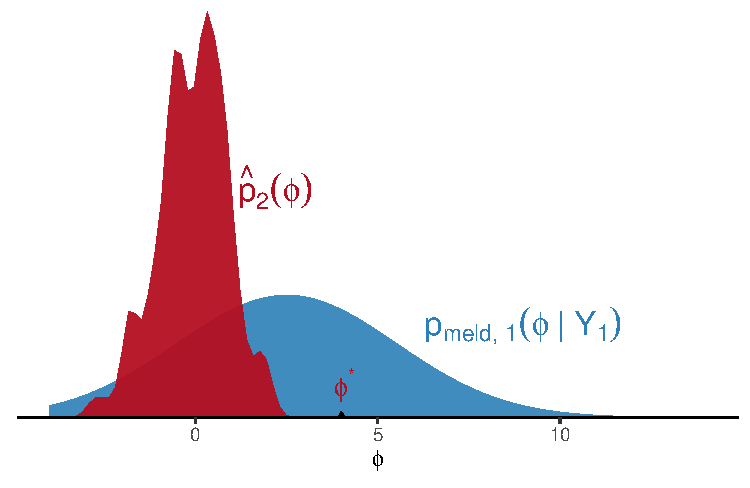
\includegraphics[width=0.85\linewidth]{figures/conflict} \end{center}

\end{frame}

\begin{frame}{\emph{Issue 1}: KDE error in action}

\begin{equation*}
  \alpha (\phi^{*}, \phi) = 
  \frac {
    \pd_{\text{pool}} (\phi^{*})
    \pd_{2}(\phi^{*}, \psi_{2}, Y_{2})
  } {
    \pd_{\text{pool}} (\phi)
    \pd_{2}(\phi, \psi_{2}, Y_{2})
  }
  \cdot
  \textcolor{myredhighlight}{
    \frac {
      \hat{\pd}_{2}(\phi)
    } {
      \hat{\pd}_{2}(\phi^{*})
    }
  }
\end{equation*}

\begin{center}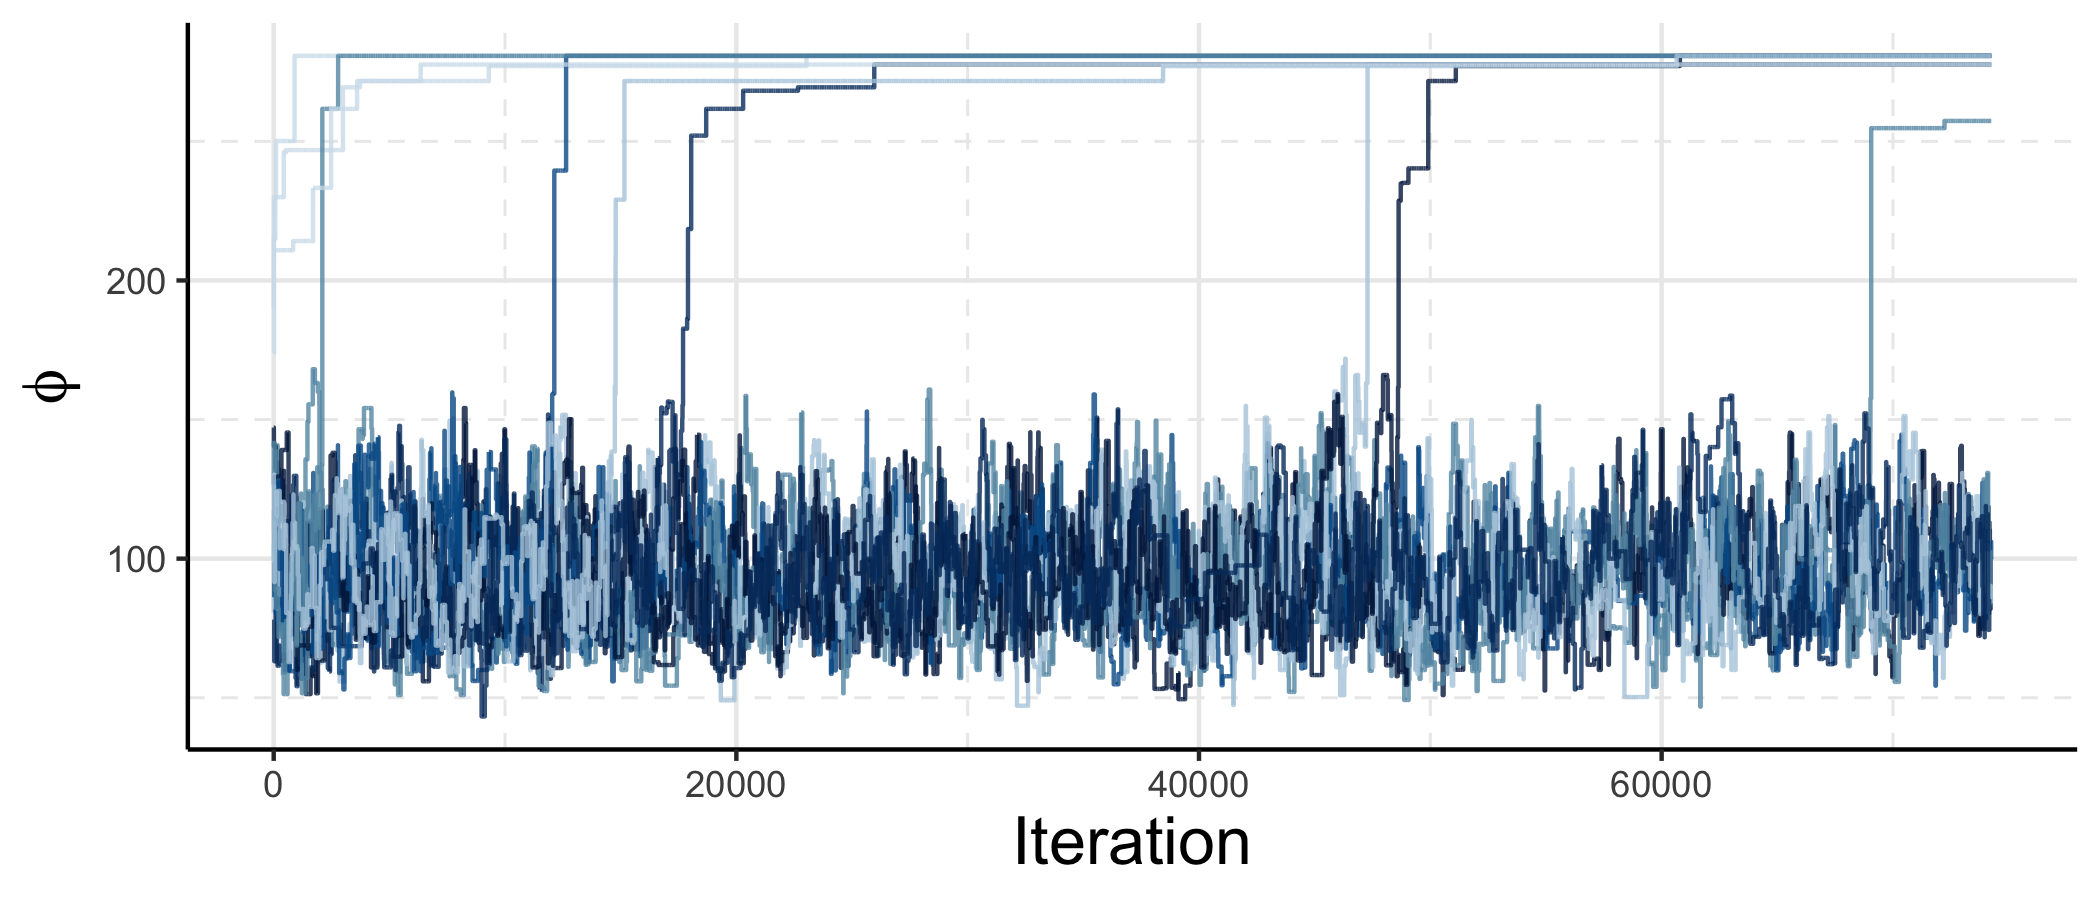
\includegraphics[width=1\linewidth]{figures/stage-two-trace-presentation-one} \end{center}

\end{frame}

\begin{frame}{\emph{Method 1}: Self density ratios}

We only interact with unknown marginal via self-density ratio (Hiraoka,
Hamada, and Hori 2018):
\begin{equation*}
  \pdr(\phinu, \phide) = \frac {
    \pd(\phinu)
  } {
    \pd(\phide)
  }
  % \label{eqn:self-densit}
\end{equation*}

\emph{Weighted-sample self-density ratio estimation} (WSRE) (Manderson
and Goudie 2020) Intuition:

\begin{itemize}
\tightlist
\item
  Sampling \(\phi \sim \pd(\phi, \psi, Y)\) admits
  \(\phi \sim \pd(\phi)\)
\item
  Instead, sample:\\
  \(\phi \sim \pd(\phi, \psi, Y) \w(\phi; \xi) \quad \rightarrow \quad \phi \sim \frac{1}{Z}\pd(\phi)\w(\phi; \xi) = \s(\phi)\)
\item
  Use the weighted sample density estimator of Jones (1991):
  \begin{equation*}
  {\textcolor{mymidblue}{\hat{\pd}}}(\phi) = 
  \frac{1}{\textcolor{mymidblue}{Z}Nh} 
    \sum\limits_{i=1}^{N} \w(\phi;\xi)^{-1} \text{K}_{h}(\phi - \phi_{i})
\end{equation*}
\item
  Ratio estimator is then: \vspace{-0.35cm}\\
  \begin{equation*}
  \pdrh(\phinu, \phide) = \frac{
    \textcolor{mymidblue}{\hat{\pd}}(\phinu)
  } {
    \textcolor{mymidblue}{\hat{\pd}}(\phide)
  }
\end{equation*}
\end{itemize}

\end{frame}

\begin{frame}{\emph{Method 1}: WSRE intuition - 1}

\begin{center}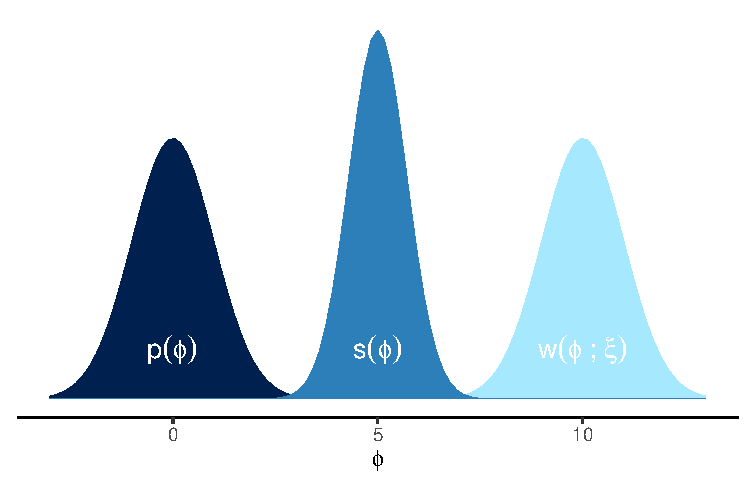
\includegraphics[width=1\linewidth]{figures/weighted-dist-plot} \end{center}

\end{frame}

\begin{frame}{\emph{Method 1}: WSRE intuition - \(\Nw\)}

\begin{center}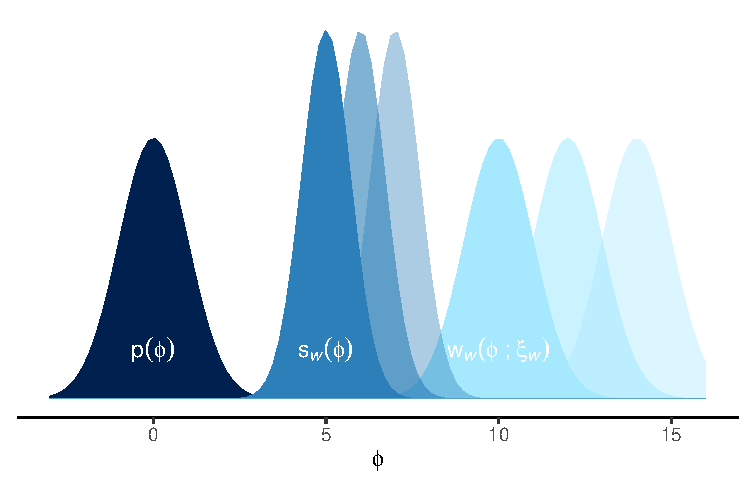
\includegraphics[width=1\linewidth]{figures/weighted-dist-plot-many} \end{center}

\end{frame}

\begin{frame}{\emph{Method 1}: H1N1 example - 2}

\begin{equation*}
  \alpha (\phi^{*}, \phi) = 
  \frac {
    \pd_{\text{pool}} (\phi^{*})
    \pd_{2}(\phi^{*}, \psi_{2}, Y_{2})
  } {
    \pd_{\text{pool}} (\phi)
    \pd_{2}(\phi, \psi_{2}, Y_{2})
  }
  \cdot
  \textcolor{mymidblue}{
    \pdrh(\phi, \phi^{*})
  }
\end{equation*}

\begin{center}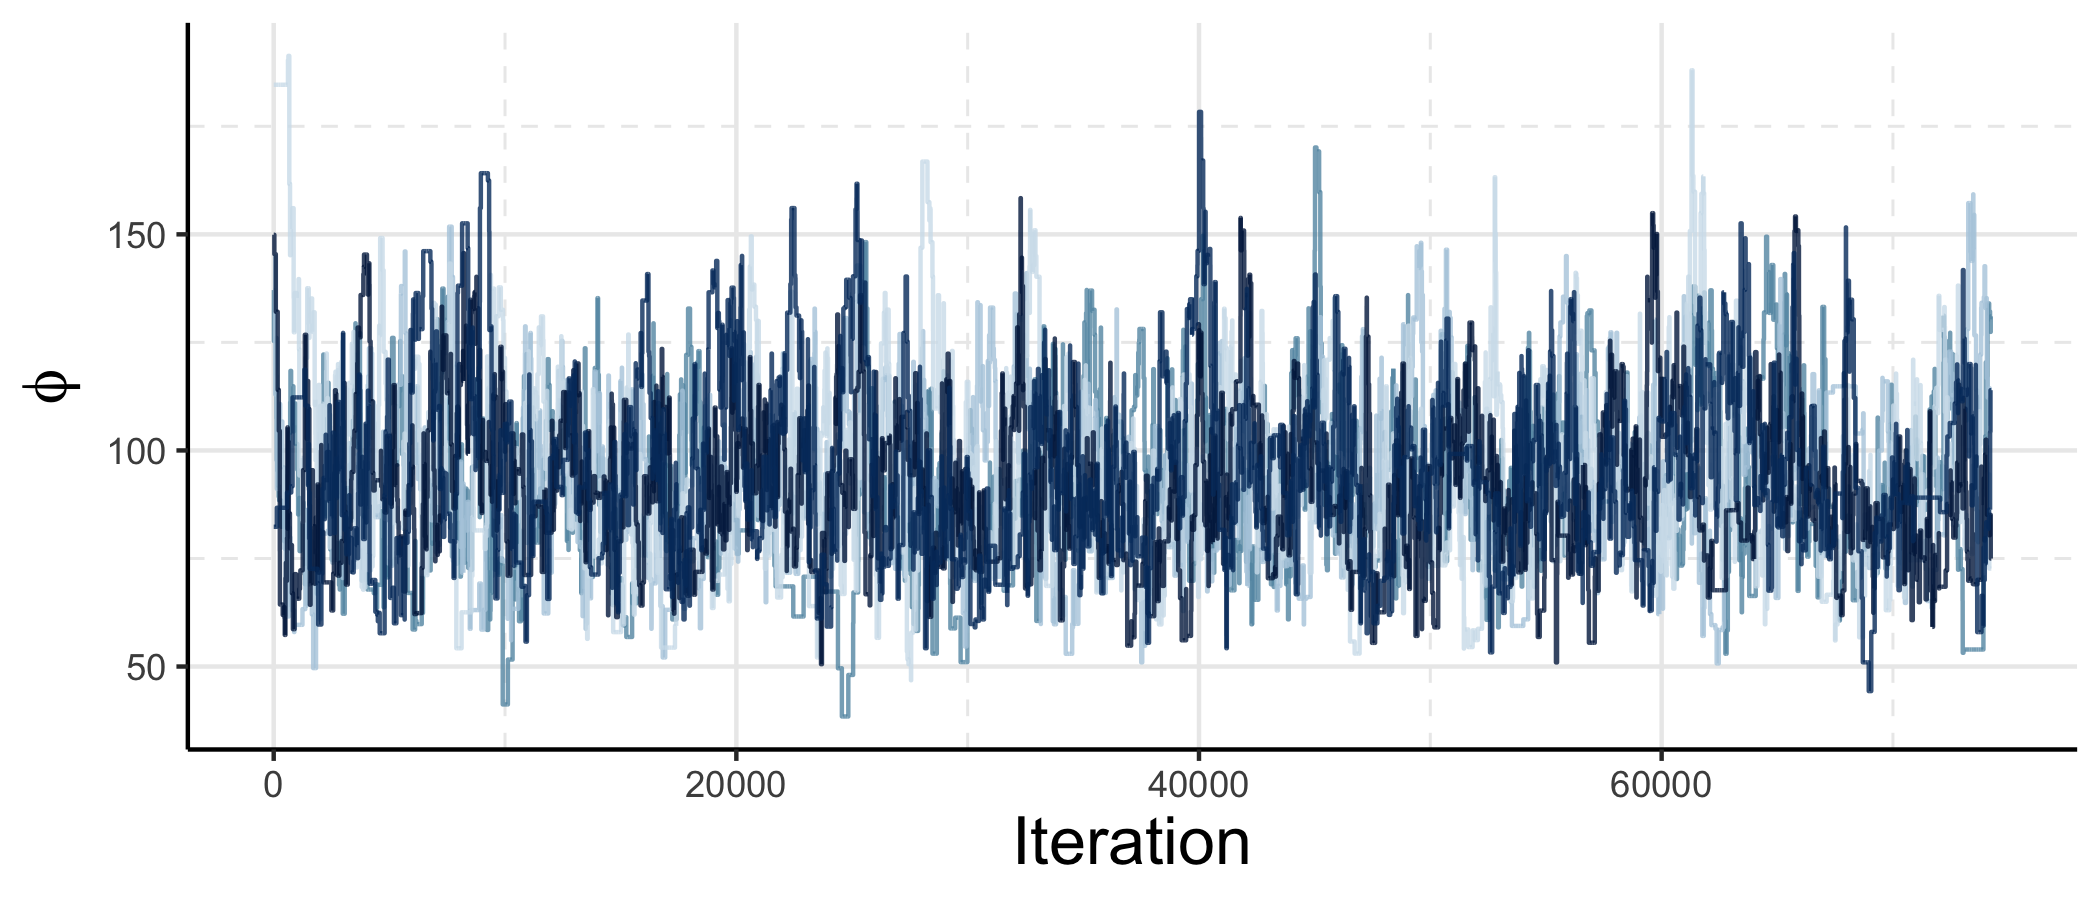
\includegraphics[width=1\linewidth]{figures/stage-two-trace-presentation-two} \end{center}

\end{frame}

\begin{frame}{\emph{Issue 2}: Submodel conflict}

\begin{center}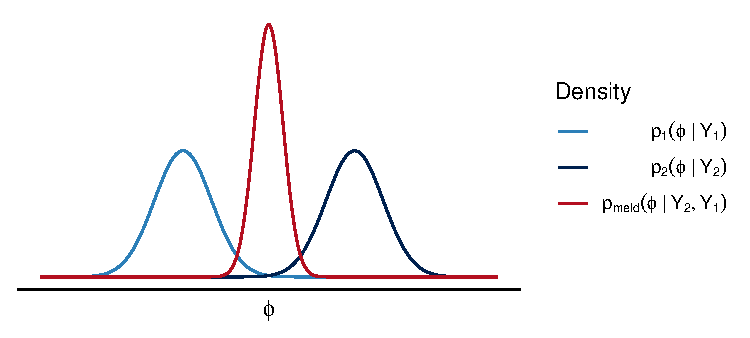
\includegraphics[width=1\linewidth]{figures/subpost-disagreement} \end{center}

\begin{itemize}
\tightlist
\item
  Last issue arose (primarily) due to differences in scale
\item
  What about more general model conflict?

  \begin{itemize}
  \tightlist
  \item
    There is a philosophical issue here
  \end{itemize}
\item
  \emph{Partial solution}: Automatic, multiple importance sampling
  (Paananen et al. 2019)
\end{itemize}

\end{frame}

\begin{frame}{\emph{Issue 3}: Multiple \(\phi\)?}

\begin{center}
\scalebox{0.8}{
\begin{tikzpicture}[> = stealth, node distance = 1.5cm, thick, state/.style={draw = none, minimum width = 1.25cm}]
  % nodes 
  \node [state] (model-1) {$\pd_{1}$};
  \node [state] [above right = of model-1] (model-3) {$\pd_{3}$};
  \node [state] [above = of model-3] (model-4) {$\pd_{4}$};
  \node [state] [below  = of model-1] (model-5) {$\pd_{5}$};

  \coordinate [above left of = model-1] (blank2);

  \node [state] [above = 2.3cm of blank2] (model-2) {$\pd_{2}$};

  % edges
  \path[->] (model-2) edge[out = 270, in = 135] node [above right] (phi-12) {$\phi_{1:2}$} (model-1);
  \path[->] (model-4) edge node [right] (phi-34) {$\phi_{3:4}$} (model-3);

  \path (model-3) edge node [below right] (phi-13) {$\phi_{1:3}$} (model-1);
  \path (model-1) edge node [right] (phi-15) {$\phi_{1:5}$} (model-5);

  % stage one - blue
  \node (stage-1) [draw = mymidblue, fit = (model-4) (phi-34), inner sep = 0.05cm, dotted] {};
  \node (stage-1-label) [yshift = 1.5ex, mymidblue] at (stage-1.north east) {$s_{1}$};
  \node (stage-1-prime) [draw = mymidblue, fit = (model-2) (phi-12), inner sep = 0.05cm, dotted] {};
  \node (stage-1-prime-label) [yshift = 1.5ex, mymidblue] at (stage-1-prime.north east) {$s_{1}'$};

  % stage two - grey
  \node (stage-2) [draw = mydarkblue, fit = (model-3) (model-4) (phi-13) (phi-34) (stage-1-label), inner sep = 0.1cm, dotted] {};
  \node (stage-2-label) [yshift = 1.5ex, mydarkblue] at (stage-2.north east) {$s_{2}$};

  % stage three - red
  \node (stage-3) [draw = myredhighlight, fit = (model-1) (model-2) (model-4) (phi-15) (phi-34) (stage-2-label), inner sep = 0.135cm, dotted] {};
  \node (stage-3-label) [yshift = 1.5ex, myredhighlight] at (stage-3.north east) {$s_{3}$};

  % stage four - black
  \node (stage-4) [draw = black, fit = (model-2) (model-4) (model-5) (phi-34) (stage-3-label), inner sep = 0.225cm] {};
  \node [yshift = 1.5ex, black] at (stage-4.north east) {$s_{4}$};

\end{tikzpicture}
}
\end{center}

\end{frame}

\begin{frame}{Conclusion}

\begin{center}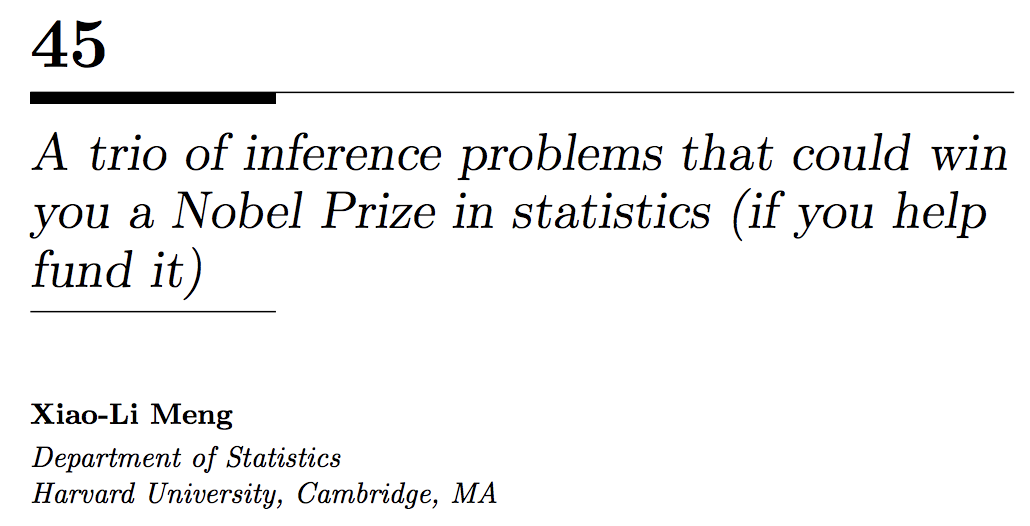
\includegraphics[width=1\linewidth]{figures/a-trio-of-inference-problems} \end{center}

\begin{itemize}
\tightlist
\item
  Multi-source inference is extremely difficult in practice (Meng 2014)
  (along with multi-resolution and multi-phase)
\end{itemize}

\end{frame}

\begin{frame}{Links}

Should you also wish to estimate self-density ratios:

\begin{itemize}
\tightlist
\item
  \url{https://github.com/hhau/wsre}
\end{itemize}

The traceplots are from this example:

\begin{itemize}
\tightlist
\item
  \url{https://github.com/hhau/full-melding-example}
\end{itemize}

This talk:

\begin{itemize}
\item ~
  \section{TODO: Push this branch to github / link to
  it}\label{todo-push-this-branch-to-github-link-to-it}
\end{itemize}

\end{frame}

\begin{frame}[allowframebreaks]{References}

\hypertarget{refs}{}
\hypertarget{ref-box:79}{}
Box, George E. P. 1979. ``Robustness in the Strategy of Scientific Model
Building.'' In \emph{Robustness in Statistics}, edited by Robert L.
Launer and Graham N. Wilkinson, 201--36. Academic Press.
doi:\href{https://doi.org/https://doi.org/10.1016/B978-0-12-438150-6.50018-2}{https://doi.org/10.1016/B978-0-12-438150-6.50018-2}.

\hypertarget{ref-box:80}{}
---------. 1980. ``Sampling and Bayes' Inference in Scientific Modelling
and Robustness.'' \emph{Journal of the Royal Statistical Society. Series
A (General)} 143 (4). Wiley: 383--430.
\url{http://www.jstor.org/stable/2982063}.

\hypertarget{ref-cook:weisberg:82}{}
Cook, R.D., and S. Weisberg. 1982. \emph{Residuals and Influence in
Regression}. Monographs on Statistics and Applied Probability. Chapman
\& Hall.

\hypertarget{ref-goudie:etal:18}{}
Goudie, Robert J. B., Anne M. Presanis, David Lunn, Daniela De Angelis,
and Lorenz Wernisch. 2019. ``Joining and Splitting Models with Markov
Melding.'' \emph{Bayesian Analysis} 14 (1). International Society for
Bayesian Analysis: 81--109.
doi:\href{https://doi.org/10.1214/18-BA1104}{10.1214/18-BA1104}.

\hypertarget{ref-hinton:02}{}
Hinton, Geoffrey E. 2002. ``Training Products of Experts by Minimizing
Contrastive Divergence.'' \emph{Neural Computation} 14 (8): 1771--1800.
doi:\href{https://doi.org/10.1162/089976602760128018}{10.1162/089976602760128018}.

\hypertarget{ref-hiraoka:hamada:hori:18}{}
Hiraoka, Kazuyuki, Toshihiko Hamada, and Gen Hori. 2018. ``Necessary and
Sufficient Conditions of Proper Estimators Based on Self Density Ratio
for Unnormalized Statistical Models.'' \emph{Neural Networks} 98:
263--70.
doi:\href{https://doi.org/10.1016/j.neunet.2017.11.018}{10.1016/j.neunet.2017.11.018}.

\hypertarget{ref-jones:91}{}
Jones, M. C. 1991. ``Kernel Density Estimation for Length Biased Data.''
\emph{Biometrika} 78 (3). Oxford University Press, Biometrika Trust:
511--19. \url{http://www.jstor.org/stable/2337020}.

\hypertarget{ref-manderson:goudie:20}{}
Manderson, Andrew A., and Robert J. B. Goudie. 2020. ``A Numerically
Stable Algorithm for Integrating Bayesian Models Using Markov Melding.''
\emph{arXiv E-Prints}, arXiv:2001.08038.

\hypertarget{ref-meng:14}{}
Meng, Xiao-Li. 2014. ``A Trio of Inference Problems That Could Win You a
Nobel Prize in Statistics (If You Help Fund It).'' CRC Press.
\url{http://nrs.harvard.edu/urn-3:HUL.InstRepos:11718181}.

\hypertarget{ref-ohagan:etal:06}{}
O'Hagan, A., C.E. Buck, A. Daneshkhah, J.R. Eiser, P.H. Garthwaite, D.J.
Jenkinson, J.E. Oakley, and T. Rakow. 2006. \emph{Uncertain Judgements:
Eliciting Experts' Probabilities}. Statistics in Practice. Wiley.
doi:\href{https://doi.org/10.1002/0470033312}{10.1002/0470033312}.

\hypertarget{ref-paananen:etal:19}{}
Paananen, Topi, Juho Piironen, Paul-Christian Bürkner, and Aki Vehtari.
2019. ``Pushing the Limits of Importance Sampling Through Iterative
Moment Matching.'' \emph{arXiv E-Prints}, arXiv:1906.08850.

\hypertarget{ref-poole:raftery:00}{}
Poole, David, and Adrian E. Raftery. 2000. ``Inference for Deterministic
Simulation Models: The Bayesian Melding Approach.'' \emph{Journal of the
American Statistical Association} 95 (452). Taylor \& Francis: 1244--55.
doi:\href{https://doi.org/10.1080/01621459.2000.10474324}{10.1080/01621459.2000.10474324}.

\end{frame}

\end{document}
